\chapter{Sixth Requirement}
\section{Analysing the relation between PSNR and Quality}
\vspace{40pt}
\begin{figure}[h]
    \centering
    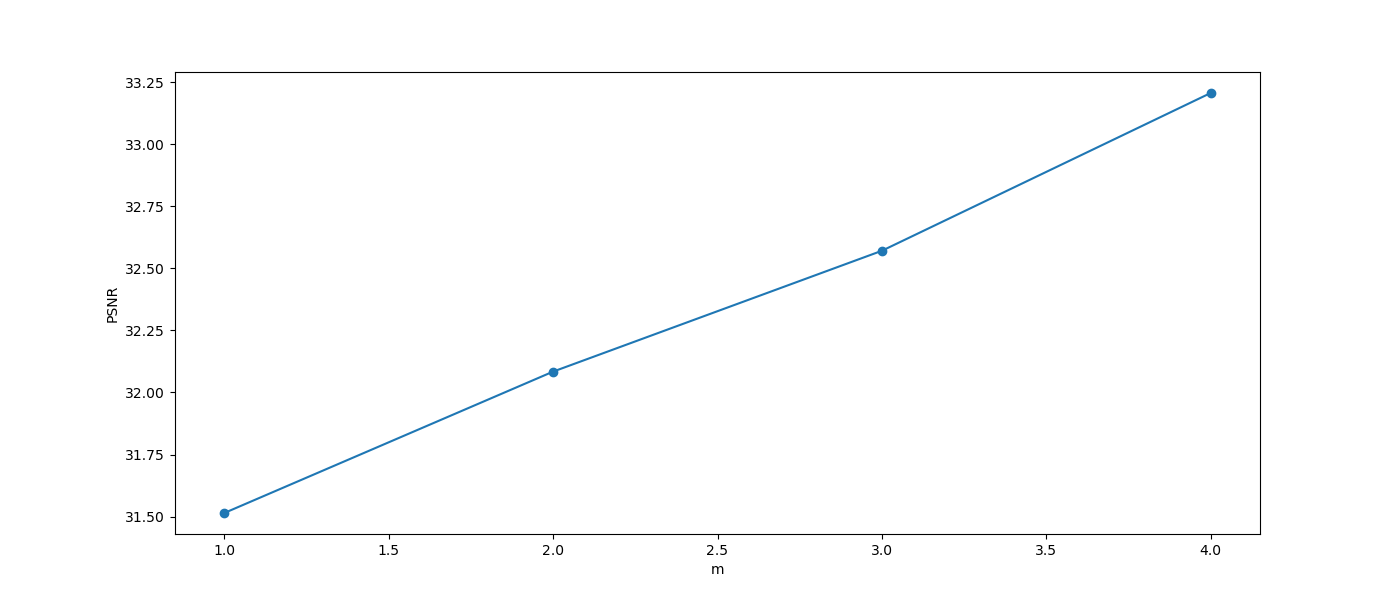
\includegraphics[width=1\textwidth]{../PSNR_plot.png}
    \caption{The Relation between $m$ and PSNR.}
    \label{fig:PSNR_m_plot}
\end{figure}


\noindent It's obvious that by increasing $m$ we take more effective frequencies,thus we enhance its quality more and more and increasing the PSNR also.
Thus the PSNR is directly propotional with $m$.